\documentclass{article}
%\documentclass[hyperref={colorlinks=true}]{beamer}
%\documentclass[handout,hyperref={colorlinks=true}]{beamer}


%%%%%%%%%%%%%%%%%%%%%%%%%%%%%%Paquetes%%%%%%%%%%%%%%%%%%%%%%%%%%%%%%%%%%%%%%%%%%%%%%%5
%%%%%%%%%%%%%%%%%%%%%%%%%%%%%%%%%%%%%%%%%%%%%%%%%%%%%%%%%%%%%%%%%%%%%%%%%%%%%%%%%%%%%
\usepackage{empheq}
\usepackage[spanish]{babel}
\usepackage[utf8x]{inputenc}
\usepackage{times}
%\usepackage[T1]{fontenc}
\usepackage{amssymb,amsmath}
\usepackage{enumerate}
\usepackage{verbatim}
\usepackage{ esint }
%\usepackage{pst-all}
%\usepackage{pstricks-add}
\usepackage{array}
%\usepackage[T1]{fontenc}
\usepackage{animate}
%\usepackage{media9}
\usepackage{xparse}
\usepackage{listings}
\usepackage{ wasysym }
\usepackage{sagetex}
\usepackage{yfonts,mathrsfs,eufrak}
\usepackage{hyperref}
\usepackage{color}
\usepackage{url}
\usepackage{theorem}
\usepackage{boiboites}


\definecolor{mygreen}{rgb}{0,0.6,0}
\definecolor{mygray}{rgb}{0.5,0.5,0.5}
\definecolor{mymauve}{rgb}{0.58,0,0.82}

\lstset{ %
  backgroundcolor=\color{white},   % choose the background color; you must add \usepackage{color} or \usepackage{xcolor}
  basicstyle=\footnotesize,        % the size of the fonts that are used for the code
  breakatwhitespace=false,         % sets if automatic breaks should only happen at whitespace
  breaklines=true,                 % sets automatic line breaking
  captionpos=b,                    % sets the caption-position to bottom
  commentstyle=\color{mygreen},    % comment style
  deletekeywords={...},            % if you want to delete keywords from the given language
  escapeinside={\%*}{*)},          % if you want to add LaTeX within your code
  extendedchars=true,              % lets you use non-ASCII characters; for 8-bits encodings only, does not work with UTF-8
  frame=single,	                   % adds a frame around the code
  keepspaces=true,                 % keeps spaces in text, useful for keeping indentation of code (possibly needs columns=flexible)
  keywordstyle=\color{blue},       % keyword style
  language=Python,                 % the language of the code
  otherkeywords={*,...},           % if you want to add more keywords to the set
  numbers=left,                    % where to put the line-numbers; possible values are (none, left, right)
  numbersep=5pt,                   % how far the line-numbers are from the code
  numberstyle=\tiny\color{mygray}, % the style that is used for the line-numbers
  rulecolor=\color{black},         % if not set, the frame-color may be changed on line-breaks within not-black text (e.g. comments (green here))
  showspaces=false,                % show spaces everywhere adding particular underscores; it overrides 'showstringspaces'
  showstringspaces=false,          % underline spaces within strings only
  showtabs=false,                  % show tabs within strings adding particular underscores
  stepnumber=2,                    % the step between two line-numbers. If it's 1, each line will be numbered
  stringstyle=\color{mymauve},     % string literal style
  tabsize=2,	                   % sets default tabsize to 2 spaces
  title=\lstname                   % show the filename of files included with \lstinputlisting; also try caption instead of title
}


%%%%%%%%%%%%%%%%%%%%%%%%%%Nuevos comandos entornos%%%%%%%%%%%%%%%%%%%%%%%%%%%%%%%%
%%%%%%%%%%%%%%%%%%%%%%%%%%%%%%%%%%%%%%%%%%%%%%%%%%%%%%%%%%%%%%%%%%%%%%%%
\newenvironment{demo}{\noindent\emph{Dem.}}{$\square$ \newline\vspace{5pt}}

\newcommand{\com}{\mathbb{C}}
\newcommand{\dis}{\mathbb{D}}
\newcommand{\rr}{\mathbb{R}}
\newcommand{\oo}{\mathcal{O}}
\renewcommand{\emph}[1]{\textcolor[rgb]{1,0,0}{#1}}
\newcommand{\der}[2]{\frac{\partial #1}{\partial #2}}
\renewcommand{\v}[1]{\overrightarrow{#1}}
\renewcommand{\epsilon}{\varepsilon}
%\newcommand{\defverbatim}{\def{#1}}
\renewenvironment{frame}[1]{}{}
\newcommand{\qed}{$\square$}
\DeclareMathOperator{\atan2}{atan2}
\DeclareMathOperator{\sen}{sen}


%%%%%%%%%%%%%%%%%%%%%%%%Colores
\definecolor{myblue}{rgb}{.8, .8, 1}
\definecolor{dblackcolor}{rgb}{0.0,0.0,0.0}
\definecolor{dbluecolor}{rgb}{0.01,0.02,0.7}
\definecolor{dgreencolor}{rgb}{0.2,0.4,0.0}
\definecolor{dgraycolor}{rgb}{0.30,0.3,0.30}
\newcommand{\dblue}{\color{dbluecolor}\bf}
\newcommand{\dred}{\color{dredcolor}\bf}
\newcommand{\dblack}{\color{dblackcolor}\bf}


%%%%%%%%%%Definimos una caja con color
\newlength\mytemplen
\newsavebox\mytempbox
\makeatletter
\newcommand\mybluebox{%
\@ifnextchar[%]
{\@mybluebox}%
{\@mybluebox[0pt]}}
\def\@mybluebox[#1]{%
\@ifnextchar[%]
{\@@mybluebox[#1]}%
{\@@mybluebox[#1][0pt]}}
\def\@@mybluebox[#1][#2]#3{
\sbox\mytempbox{#3}%
\mytemplen\ht\mytempbox
\advance\mytemplen #1\relax
\ht\mytempbox\mytemplen
\mytemplen\dp\mytempbox
\advance\mytemplen #2\relax
\dp\mytempbox\mytemplen
\colorbox{myblue}{\hspace{1em}\usebox{\mytempbox}\hspace{1em}}}
\makeatother
\DeclareDocumentCommand\boxedeq{ m g }{%
{\begin{empheq}[box={\mybluebox[2pt][2pt]}]{equation}% #1%
\IfNoValueF {#2} {\label{#2}}%
#1
\end{empheq}
}%
}


%%%%%%%%%%%%%%%%%%
\newboxedtheorem[boxcolor=orange, background=blue!5, titlebackground=blue!20,
titleboxcolor = black,thcounter=section]{problema}{Problema}{thcounter1}

\newboxedtheorem[boxcolor=orange, background=blue!5, titlebackground=blue!20,
titleboxcolor = black,thcounter=section]{teorema}{Teorema}{thcounter2}

\newboxedtheorem[boxcolor=orange, background=blue!5, titlebackground=blue!20,
titleboxcolor = black,thcounter=section]{definicion}{Definici\'on}{thcounter3}

\newboxedtheorem[boxcolor=orange, background=blue!5, titlebackground=blue!20,
titleboxcolor = black,thcounter=section]{lema}{Lema}{thcounter4}

\newboxedtheorem[boxcolor=orange, background=blue!5, titlebackground=blue!20,
titleboxcolor = black,thcounter=section]{corolario}{Corolario}{thcounter5}

\newboxedtheorem[boxcolor=orange, background=blue!5, titlebackground=blue!20,
titleboxcolor = black,thcounter=section]{proposicion}{Proposici\'on}{thcounter6}

\newboxedtheorem[boxcolor=orange, background=blue!5, titlebackground=blue!20,
titleboxcolor = black,thcounter=section]{codigo}{Función SymPy}{}



        {\theorembodyfont{\normalfont}
\newtheorem{ejemplo}{Ejemplo}}


%%%%%%%%%%%%%%%%%%%%%%%%%%%%%%%%%%%%%%%%%%%%%%%%%%%%%%%%%%%%%%%%%%%%%%%%%%%%%%%%%%%%%%%%%%%%%%%%%%%%%%%%%%%
%%%%%%%%%%Para escibir en clase articulo o similar






\title{Generalidades}
\author{Fernando Mazzone}

%%%%%%%%%%%%%%%%%%%%%%%%%%%%%%%%%%%%%%%%%%%%%%%%%%%%%%%%%%%%%%%%%%%%%%%%%%%%%%%%%%%%%%


\begin{document}
  \maketitle
\tableofcontents


















\section{Sobre esta materia}

\begin{itemize}
 \item  \href{https://docs.google.com/viewer?a=v&pid=sites&srcid=ZGVmYXVsdGRvbWFpbnxlY3VhY2lvbmVzZGlmZXJlbmNpYWxldW5yY3xneDoyZjE0YzJmMDcyODc0ZGQ3}{Programa analítico.}
 \item  \href{https://sites.google.com/site/ecuacionesdiferencialeunrc/ecuaciones-diferenciales-unrc}{Página web} de la materia
 \item  Vamos a hacer uso intensivo de paquetes de matemática basados en \href{https://www.python.org/}{Python}, por ejemplo \href{http://www.scipy.org/}{SciPy},  \href{http://www.scipy.org/}{SymPy} y \href{http://www.sagemath.org/}{SAGE}.
 \item  Requeriremos muchos contenidos de la asignatura Física.
 \item  \begin{tabular}{m{4cm} m{2cm} m{2cm}} Bibliografía principal & 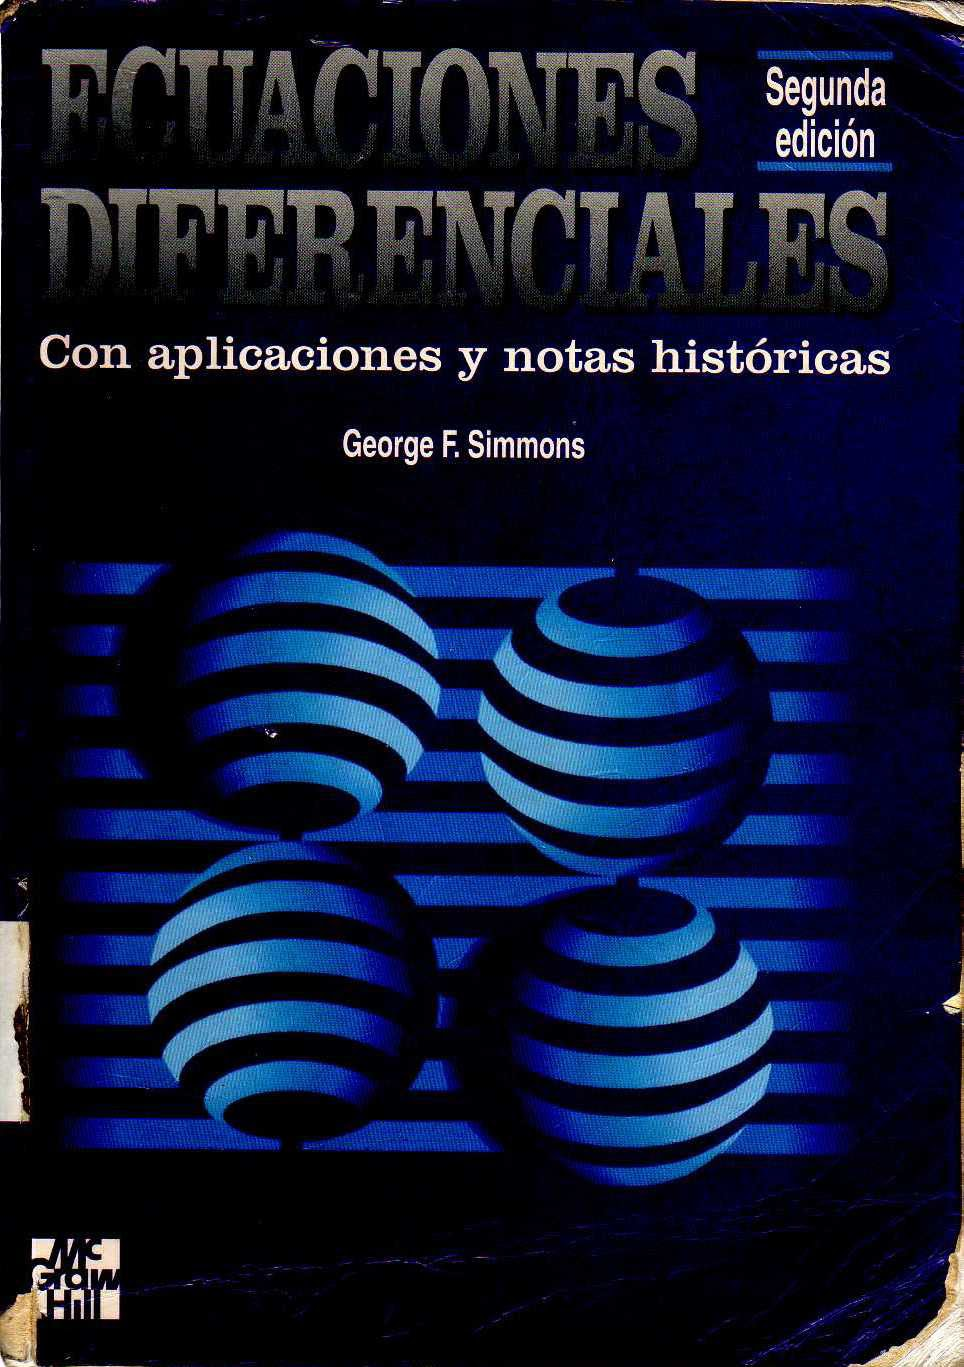
\includegraphics[scale=0.05]{imagenes/Tapa_Simmons.jpg} &    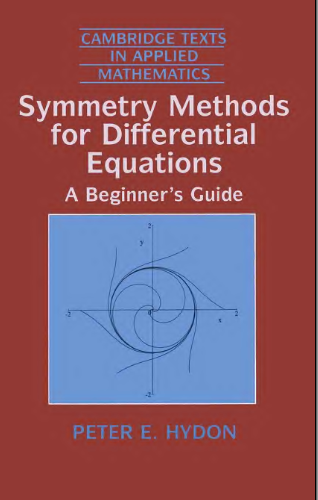
\includegraphics[scale=0.13]{imagenes/tapa_hydon.png}          \end{tabular}

\end{itemize}



\section{¿Que son las ecuaciones diferenciales?}


\begin{definicion}[Ecuación diferencial, definición informal]
 Es una o varias relaciones entre una o varias variables dependientes y sus tasas de cambio respecto a ciertas variables independientes.
 \end{definicion}

 El problema básico asociado
 a las ecuaciones diferenciales es hallar las variables dependientes que las resuelven.

 Las ecuaciones diferenciales son usadas muy a menudo en matemática aplicada, puesto que muchas
 leyes (de la física por ejemplo) se expresan atraves de este tipo de ecuaciones.








 \begin{ejemplo}[\href{http://es.wikipedia.org/wiki/Caída_libre}{Caída libre}] Modelizar matemáticamente el movimiento de un cuerpo de masa $m$ en las proximidades de la superficie
terrestre, asumiendo que su movimiento es
sobre la vertical y que las fuerzas que sobre él actúan son la gravedad y el rozamiento con el aire.
\end{ejemplo}
 \begin{tabular}{m{4.5cm} m{5cm}} 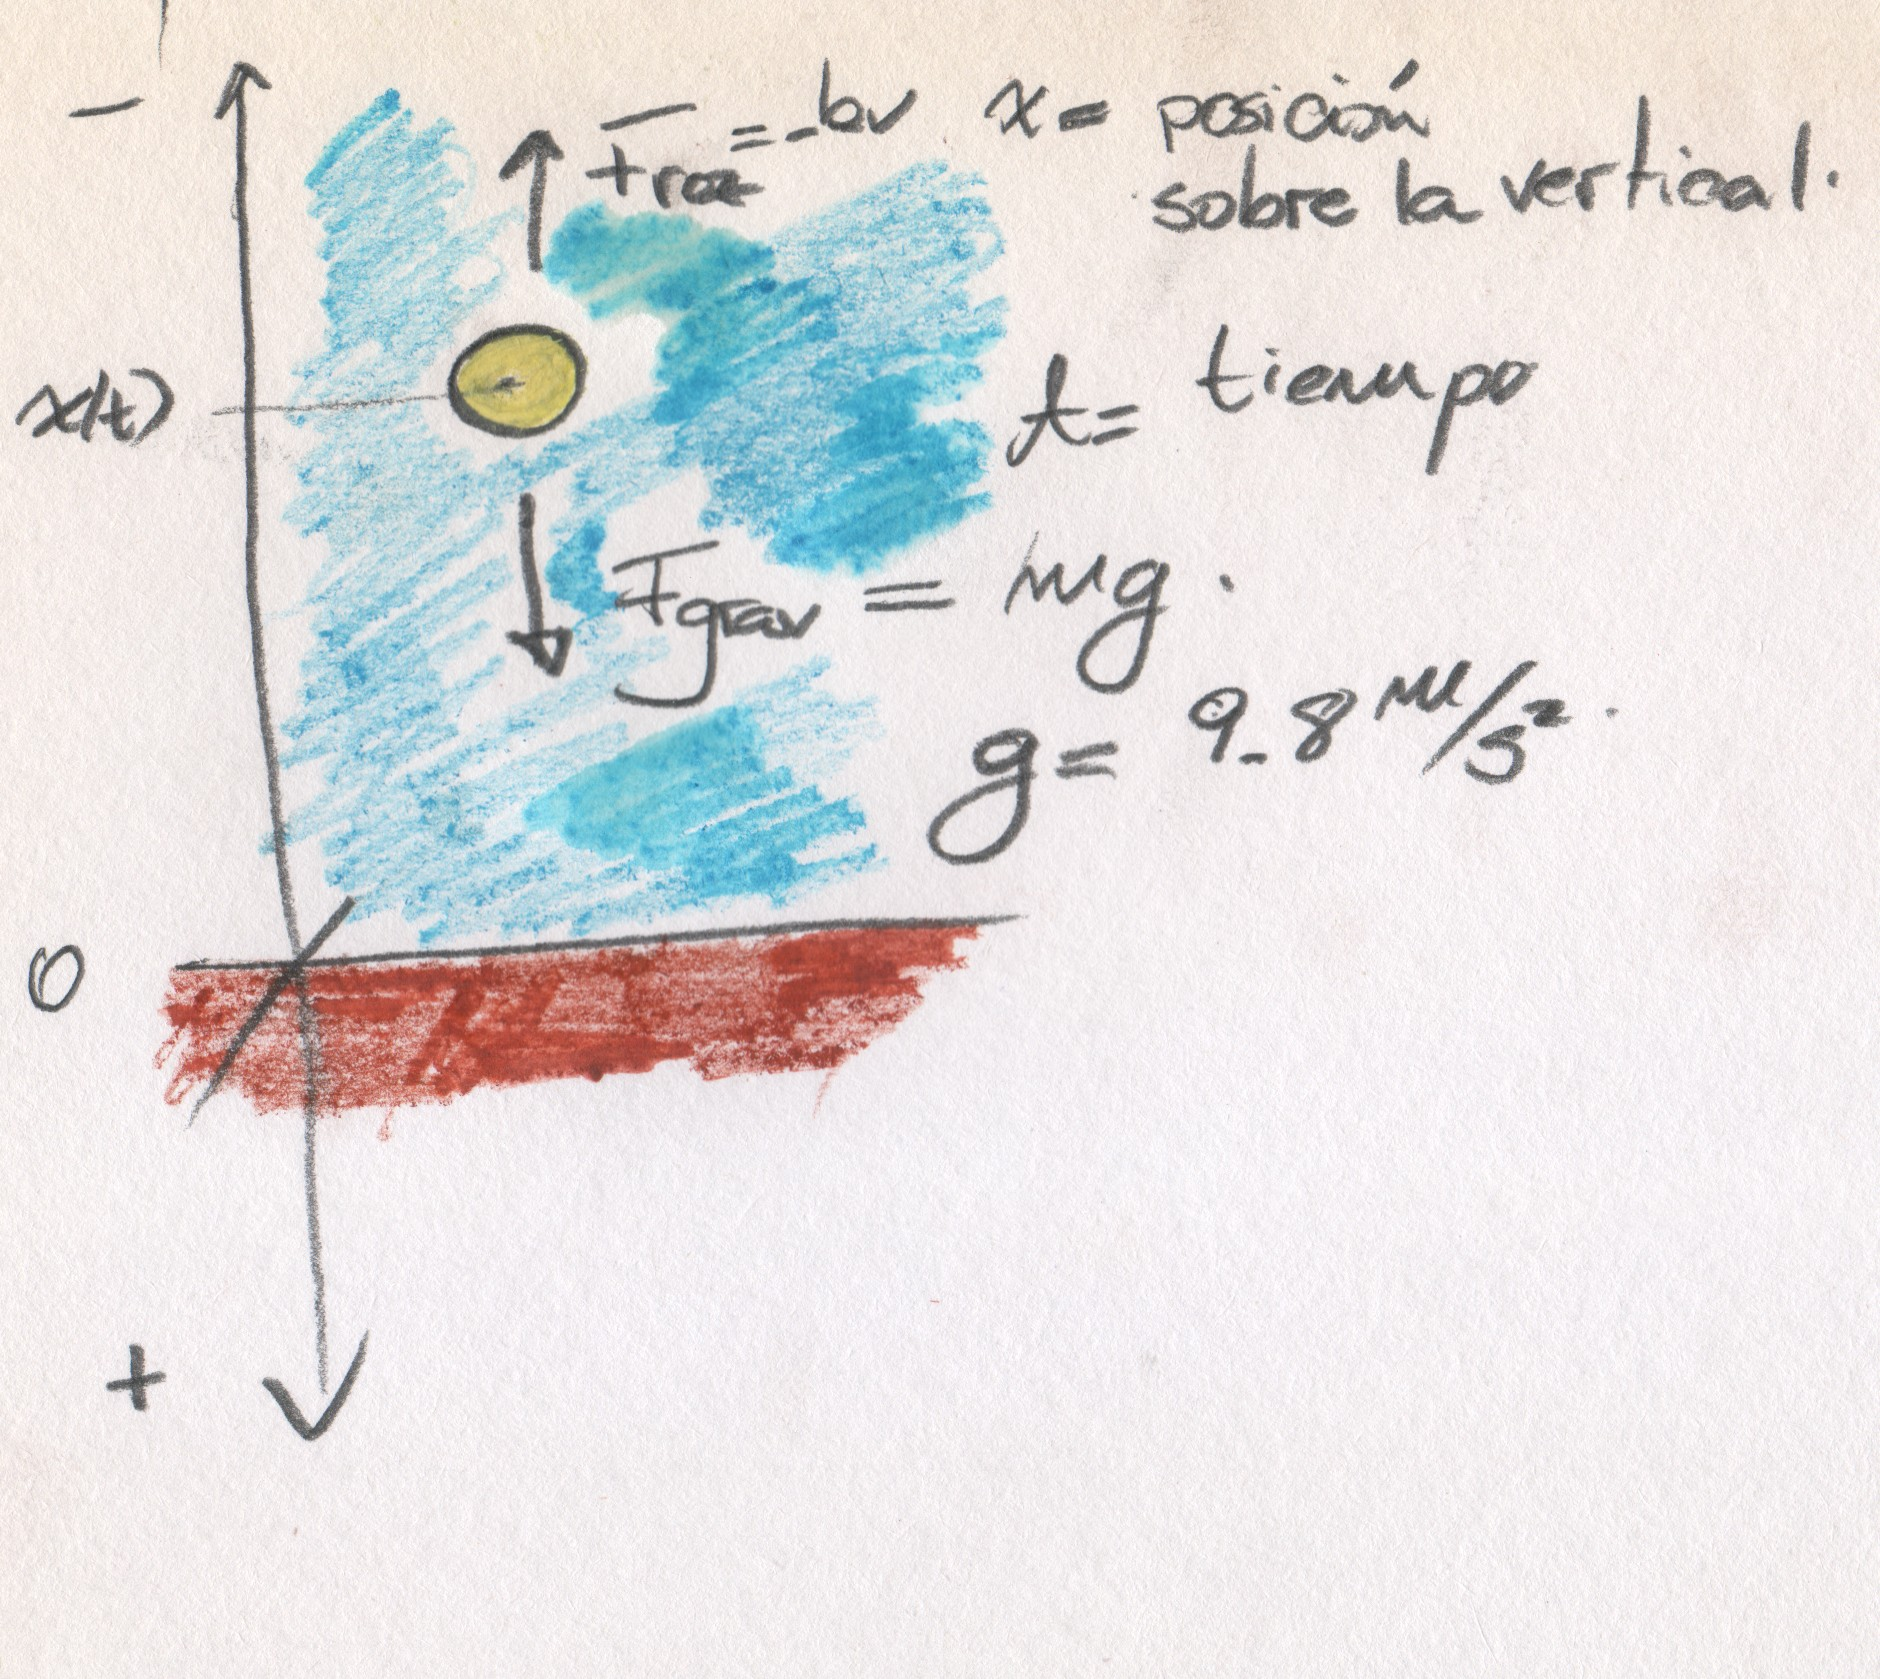
\includegraphics[scale=0.07]{imagenes/caida_libre.jpg}    &  $x(t)=$ posición a lo largo de la vertical, relativo a un eje de coordenadas\newline
$v(t)=\frac{dx}{dt}=$ velocidad\newline
$F_{grav}=$ fuerza debida a la gravedad $=mg$ donde $g=9.8m/s^2$
$F_{roz}=$ fuerza de rozamiento, proporcional a la velocidad y de sentido contrario $=-cv$, $c>0$.

\end{tabular} 



 Usamos la \href{http://es.wikipedia.org/wiki/Leyes_de_Newton}{Segunda Ley de Newton}, esto es la suma de las fuerzas totales que actuan sobre un cuerpo de masa $m$
es igual al producto de la masa $m$ y la aceleración $a(t)$. Recordemos que la aceleración es la tasa de cambio de la velocidad, es decir la derivada segunda de la posición.   

  Usando todas las relaciones mencionadas

\[ma(t)=mv'(t)=F_{\hbox{total}}=F_{\hbox{grav}}+F_{\hbox{roz}}=mg-cv\]

vale decir
\begin{equation}\label{caidaLibre1}
 \boxed{ x''(t)+\frac{c}{m} x'(t)=g.}
\end{equation}
\begin{equation}\label{caidaLibre2}
\boxed{ v'(t)+\frac{c}{m} v=g.}
\end{equation}





\section{Algunos conceptos relacionados con ecuaciones diferenciales}

\begin{definicion}[Orden] El índice de la mayor derivada interviniente en la ecuación.
 \end{definicion}

 Por ejemplo la ecuación \eqref{caidaLibre1} es de orden 2 y la
ecuación \eqref{caidaLibre2}, si bien está estrechamente relacionada con la anterior, es de orden 1. Como regla casi general, cuanto menor es el orden,  más fáciles de estudiar y/o resolver las ecuaciones son.

  \begin{definicion}[Solución] Una función que satisface la relación que indica la ecuación.

   \end{definicion}

   Por ejemplo
\begin{equation}\label{SolGencaidaLibre2} v(t)=\frac{m}{c}g+ke^{-\frac{c}{m}t},\end{equation}
resuelve \eqref{caidaLibre2}, para todo $C\in\rr$. No deberíamos perder tiempo en chequear una cuestión tan sencilla, pero aprovechemos la ocasión para usar  \href{http://www.sympy.org}{SymPy}.





\begin{lstlisting}
>>>from sympy import *
>>>m,g,c,k,t=symbols('m,g,c,k,t')
>>>v=m/c*g+k*exp(-c/m*t)
>>>simplify(v.diff(t)+c/m*v)
g
\end{lstlisting}
Notar que las líneas que comienzan con el signo del prompt \verb~>>>~ indican entradas por línea de comandos y las que comienzan sin este signo son las respuestas del interprete.

Rara vez utilizaremos las siguientes funcionalidades de sympy, pero es oportuno decir que
 \texttt{SymPy} puede encontrar la solución a una ecuación diferencial

\begin{lstlisting}
>>>v=symbols('v',cls=Function)
>>>EqCaida=Eq(v(t).diff(t)+c/m*v(t),g)
>>>Vel=dsolve(EqCaida,v(t))
>>> Vel
v(t) == (g*m + exp(c*(C1 - t/m)))/c
\end{lstlisting}

La solución obtenida es la ya conocida. Es instructivo averiguar que tipo de dato tiene la variable \verb~Vel~

\begin{lstlisting}
>>> type(Vel)
<class 'sympy.core.relational.Equality'>
\end{lstlisting}
A este tipo de cuestiones hay que prestar atención cuando se trabaja con sympy, pues existe la tendencia a confudir los conceptos matemáticos con los propios del lenguaje. Por ejemplo, matemáticamente una solución es una función. Sin embargo, en este caso, cuando le solicitamos una solución a sympy nos entrega un objeto de tipo  ``relación de igualdad``.





\begin{definicion}[Ecuación diferencial ordinaria (EDO)] Es una ecuación donde las variables dependientes sólo dependen de una única variable independiente.
\end{definicion}

Las
ecuaciones \eqref{caidaLibre1} y \eqref{caidaLibre2} son ejemplo de ello, la variable independiente es el tiempo.
  \begin{definicion}[Ecuación en derivadas parciales (EDP)] Es una ecuación donde las variables dependientes dependen de más de una variable independiente.
   \end{definicion}

Ejemplo de este tipo de ecuación es la ecuación de Laplace

\[\frac{\partial^2 u}{\partial x^2}+\frac{\partial^2 u}{\partial y^2}=0\]

Puede ocurrir también que dispongamos de varias ecuaciones diferenciales que se deben satisfacer simultaneamente. En estos casos, el conjuntos de ecuaciones se suele escribir como una única ecuación vectorial. Por este motivo, muchas veces, cuando dispongamos de una única ecuación diremos que tenemos una \emph{ecuación  escalar}.

\begin{definicion}[Sistema de ecuaciones] Es un  conjunto de ecuaciones diferenciales que se deben satisfacer simultaneamente.
 \end{definicion}

En ese caso es  de esperar que tengamos varias incognitas en
nuestro problema. En general una ecuación escalar determina sólo una incognita. De hecho aquí ocurre, a semejanza con ecuaciones algebraicas, que es frecuente necesitar tantas ecuaciones como incognitas.

\begin{ejemplo}[Ecuación del péndulo] El sistema de ecuaciones:
\[\left\{ \begin{array}{l l} x'&=y \\y'&=-\sen(x) \end{array}\right.\]
es muy conocido pues modeliza el movimiento de un péndulo.
\end{ejemplo}



Muy a menudo hablaremos de resolver una ecuación, pero es oportuno discutir que queremos significar con esto.

\begin{definicion}[Resolver una ecuación] Es expresar la solución como combinaciones algebraicas y composiciones de funciones que consideramos elementales.
\end{definicion}

Esta definición contiene una vaga apelación a ciertas ``funciones elementales''. El universo de funciones que se considera elemental es una cuestión política, no matemática. En  principio, consideraremos elementales a las potencias, exponenciales, logarítmos, trigonométricas y trigonométricas inversas. No obstante esta lista se puede expandir con muchas funciones especiales.  Las operaciones permitidas para combinar estas funciones
también están sujetas a convenciones. Por ejemplo, admitiremos como válida una expresión que contenga una integral, al menos en el caso que no sea claro como resolver esta integral.

 Casi todo este curso trata con la discusión de métodos para resolver ecuaciones.  Sin embargo resolver ecuaciones no es quizás el problema principal relacionado con las ecuaciones diferenciales. No importa tanto lograr una expresión formal de la solución, como, por ejemplo, conocer las propiedades que poseen las soluciones. Al fin y al cabo, uno conoce una función a través de sus propiedades.
 





\begin{definicion}[Solución general] Usualmente una ecuación presenta infinitas soluciones. Una solución general  es una expresión que representa todas estas soluciones. Es habitual que una solución general contenga parámetros. Cada elección de estos parámetros determina una solución distinta.
 \end{definicion}

 Por ejemplo \eqref{SolGencaidaLibre2} es la solución general de \eqref{caidaLibre2}.
  La afirmación anterior requiere una demostración puesto que sólo hemos mostrado que \eqref{SolGencaidaLibre2} es solución, pero no
que toda solución se expresa con \eqref{SolGencaidaLibre2}. Para demostrar la afirmación, hay que multiplicar ambos miembros de \eqref{caidaLibre2} 
por $e^{\frac{c}{m}t}$ y luego integrar respecto a $t$ 
\[\frac{mg}{c}e^{\frac{c}{m}t}=\int ge^{\frac{c}{m}t}dt=\int v'(t)e^{\frac{c}{m}t}+\frac{c}{m}e^{\frac{c}{m}t} vdt=e^{\frac{c}{m}t}v+C.\]
 Despejando $v$ del primer y último miembro obtenemos \eqref{SolGencaidaLibre2} con $k=-C$.

 




\begin{ejemplo} En algunas ocasiones sólo podemos dejar una relación implícita entre las variable dependientes e independientes. Por ejemplo
\begin{equation}\label{solImpl}x=e^y+y+C\quad\text{ para } C\in\rr\end{equation}
es solución general de
\[y'(e^y+1)=1.\]
Vamos a chequear sólo que \eqref{solImpl} es solución, dejando la justificación que toda solución tiene esa forma para más adelante. Derivando \eqref{solImpl}
\[ 1=e^yy'+y'\]
Luego $y'=1/(1+e^{y})$. Reemplazando esta relación  en la ecuación diferencial corroboramos que es solución.
\end{ejemplo}



\section{Definición formal}

\begin{definicion}[Ecuación diferencial] Una ecuación diferencial ordinaria de orden $n$ es una relación de la forma
\[\boxed{F(x,y(x),y'(x),\ldots,y^{(n)}(x))=0}.\]
donde $F:(a,b)\times \Omega\to\rr$, $\Omega$ es abierto de $\rr^{n+1}$ y $(a,b)$ un intervalo de $\rr$.
  \end{definicion}





\begin{ejemplo} El problema de hallar una primitiva de una función es una ecuación diferencial que, como ya has visto en cursos iniciales de análisis, se relaciona con el concepto de integral. Supongamos $f:(a,b)\subset \rr\to\rr$ una función continua. Consideremos la ecuación diferencial
\[y'(x)=f(x).\]
Sea $x_0\in(a,b)$, integrando respecto a $x$ entre $x_0$ y $x$
\[y(x)=y(x_0)+\int_{x_0}^xf(t)dt\]
Que es una solución general. Quedaría determinada una única solución si, por ejemplo, conociecemos $y(x_0)$.
\end{ejemplo}



\begin{ejemplo} Supongamos $f:(a,b)\subset \rr\to\rr$ como antes. Consideremos la ecuación diferencial
\[y''(x)=f(x).\]
Tomemos una integral indefinida respecto a $x$ 
\[y'(x)=C_1+\int f(t)dt\]
Ahora deberemos tomar una integral indefinida más
\[y(x)=C_2+C_1t +\int\left(\int f(x)dx\right)dx.\]
Ahora quedan dos constantes $C_1$ y $C_2$. 
\end{ejemplo}



 \begin{definicion}[Principio de Hadamard]
 Un problema se dice \href{http://es.wikipedia.org/wiki/Problema_bien_definido}{bien planteado} segun Hadamard si satisface que
 \begin{enumerate}
  \item El problema admite solución
  \item La solución es única
  \item La solución depende de manera continua de los datos numéricos del problema.
 \end{enumerate}
\end{definicion}

 Como hemos visto, una ecuación diferencial no determina una única solución, por consiguiente no sería un problema bien planteado. Debemos agregar relaciones
a nuestro problema para que sea bien planteado. Es así que aparecen condiciones iniciales, problemas de contorno, etc.
 




\begin{definicion}[Problemas de valores iniciales] Sea $x_0\in(a,b)$, $F:(a,b)\times \Omega\to\rr$ e $y_0,y_0^1,\ldots,y_0^{n-1}\in\rr$. Las siguientes relaciones  se denominan problema de
valores iniciales
\[
 \left\{\begin{array}{l l l}
         F(x,y,y',&\ldots,y^{(n)})=0& x\in(a,b)\\
         y(x_0)&=y_0&\\
         y'(x_0)&=y_0^1&\\
          & \vdots &\\
          y^{(n-1)}(x_0)&=y_0^{n-1}&\\
        \end{array}
   \right.
\]

\end{definicion}



\begin{definicion}[Ecuaciones de primer orden] La ecuación general de primer orden tiene la forma
\[
F(x,y(x),y'(x))=0,
\]
donde $F:(a,b)\times \Omega\to\rr$ y $\Omega$ abierto de $\rr^2$. Con frecuencia asumiremos que $y'$ se despeja de la relación anterior, es decir que existe $f:\Omega'\to\rr$,
$\Omega'$ abierto de $\rr^2$, tal que
\[y'=f(x,y).\]
Bajo esta suposición, si $(x_0,y_0)\in\Omega'$ el problema de valores iniciales se escribe
\[\left\{\begin{array}{l l}
	    y'&=f(x,y)\\
	    y(x_0)&=y_0
         \end{array}\right.
\]
\end{definicion}



\section{Familias paramétricas de funciones}

En las secciones siguientes vamos a describir problemas, matemáticos y físicos que se reducen a un problema de ecuaciones diferenciales.


\begin{problema}
Dada una familia paramétrica de funciones
 \begin{equation}\label{flia_param}y=y(x,c),\end{equation}
 dependiente del parámetro $c\in\rr$, ¿Será posible hallar una ecuación para la cual la familia sea la solución general?
\end{problema}


{Familias paramétricas de funciones}
En líneas generales la respuesta es si. Nos conviene expresar \eqref{flia_param} como una ecuación implícita
\begin{equation}\label{flia_impl}f(x,y,c)=0.\end{equation}
Derivando esta ecuación respecto a $x$
\begin{equation}\label{der_impl}
 \frac{\partial f}{\partial x}+\frac{\partial f}{\partial y}y'(x,c)=0.
\end{equation}
Ahora es posible eliminar $c$ de \eqref{flia_impl} y \eqref{der_impl} al costo de quedarnos con una sola ecuación.




\begin{ejemplo} Encontrar la ecuación que satisface la familia paramétrica
\[x^2+y^2=c^2.\]
Derivamos
\[2x+2yy'=0.\]
Ya está!!!
\end{ejemplo}

\begin{ejemplo} Idem $x^2+y^2=2cx$.  Derivando
\[2x+2yy'=2c.\]
Eliminamos $c$ de las dos relaciones
\[\frac{x^2+y^2}{x}=2x+2yy'\Rightarrow \boxed{y'=\frac{y^2-x^2}{2xy}}.\]
\end{ejemplo}


\begin{problema}
 Dada una familia paramétrica
 \[f(x,y,c)=0,\]
 encontrar otra
 \[g(x,y,d)=0\]
 tal que los ángulos que forman los gráficos entre las funciones de una y de otra familia sean rectos  en cada punto de corte entre ellos.
\end{problema}




Para resolver este problema se completan estos pasos
\begin{itemize}
 \item Se encuentra la ecuación diferencial que satisface la familia dada, digamos
 \[y'=h(x,y).\]
 \item Se resuelve
 \[y'=-\frac{1}{h(x,y)}.\]
\end{itemize}




\begin{ejemplo} Encontrar la familia de curvas ortogonales a la flia de circunferencias

\[x^2+y^2=c^2\]

Hallamos antes que la ecuación que satisfacen estas curvas es
\[y'=-\frac{x}{y}.\]
Luego deberíamos resolver
\[y'=\frac{y}{x}.\]
Que no sabemos pero SymPy si!!!

\end{ejemplo}

\begin{codigo}[\texttt{dsolve}]

\textbf{Sintaxis} (\href{http://docs.sympy.org/latest/modules/solvers/ode.html#}{documentación \texttt{SymPy}})

\texttt{dsolve(eq, f(x), hint)}

\texttt{eq:} Ecuación (posicional)

\texttt{f(x):} función incognita (posicional)

\texttt{hint: } Método a emplear. Argumento con nombre \texttt{hint='cadena'}.

\end{codigo}

\begin{ejemplo}
\end{ejemplo}
\begin{lstlisting}
x=symbols('x')
y=Function('y')(x)
MiEcua=Eq(y.diff(x),y/x)
f=dsolve(MiEcua,y)
\end{lstlisting}

\noindent\textbf{Resultado:}
Flía rectas  por el origen. \\
La instrucción\\
\texttt{f=dsolve(MiEcua,y,hint='separable')}
\\produce el mismo resultado.






\begin{codigo}[\texttt{plot}]

\textbf{Sintaxis} (\href{http://docs.sympy.org/latest/modules/plotting.html}{documentación \texttt{SymPy}})

Para un gráfico simple

\texttt{plot(expr,rango,opcionales(claves))}

\texttt{expr:} Expresión a graficar 

\texttt{rango:} Conjunto donde varia la variable independiente 

\texttt{opcionales } Argumentos que modifican la apariencia del gráfico. Generalemente de la forma de clave=valor

\end{codigo}


\begin{ejemplo}

\end{ejemplo}


\begin{lstlisting}
x=symbols('x')
f=plot(1/x,(x,-3,3),ylim=(-3,3))
\end{lstlisting}

\noindent\textbf{Resultado:}
\begin{center}
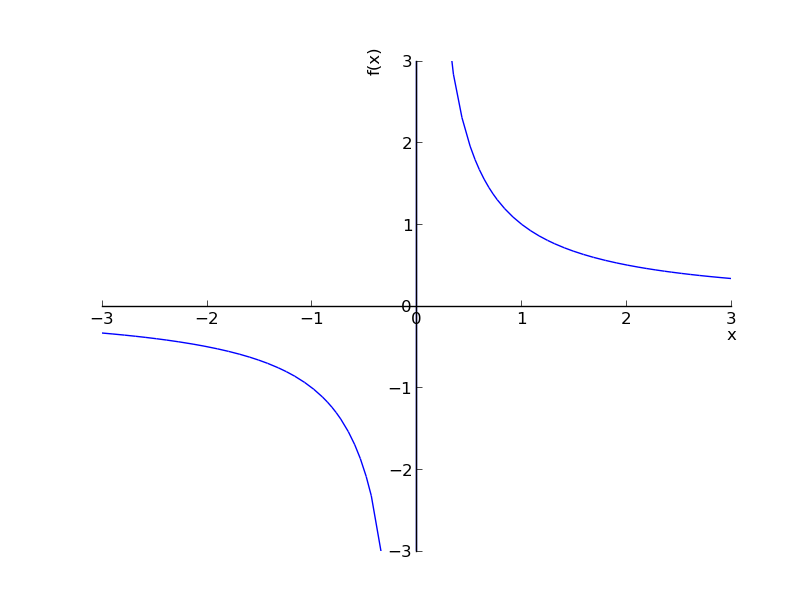
\includegraphics[scale=.35]{imagenes/ejemplo_plot.png}
\end{center}












\begin{ejemplo}Grafiquemos un familias paramétrica de funciones.

\end{ejemplo}




\begin{lstlisting}
from sympy import *
x,y=symbols('x,y')
Rango=range(21)
L=[tan(pi*k/21.0) for k in Rango] 
p=plot(L[0]*x,(x,-2,2),show=False,xlim=(-2,2),\
ylim=(-2,2),aspect_ratio=(1,1))
for pend in L[1:]:
    p1=plot(pend*x,(x,-2,2),show=False,\
xlim=(-2,2),ylim=(-2,2),aspect_ratio=(1,1))
    p.append(p1[0])
for r in range(1,10):
    p1=plot_implicit(Eq(x**2 + y**2, 0.2*r),\
show=False,aspect_ratio=(1,1),xlim=(-2,2),ylim=(-2,2))
    p.append(p1[0])
\end{lstlisting}


\noindent\textbf{Resultado:}
\begin{figure}[h]
\begin{center}
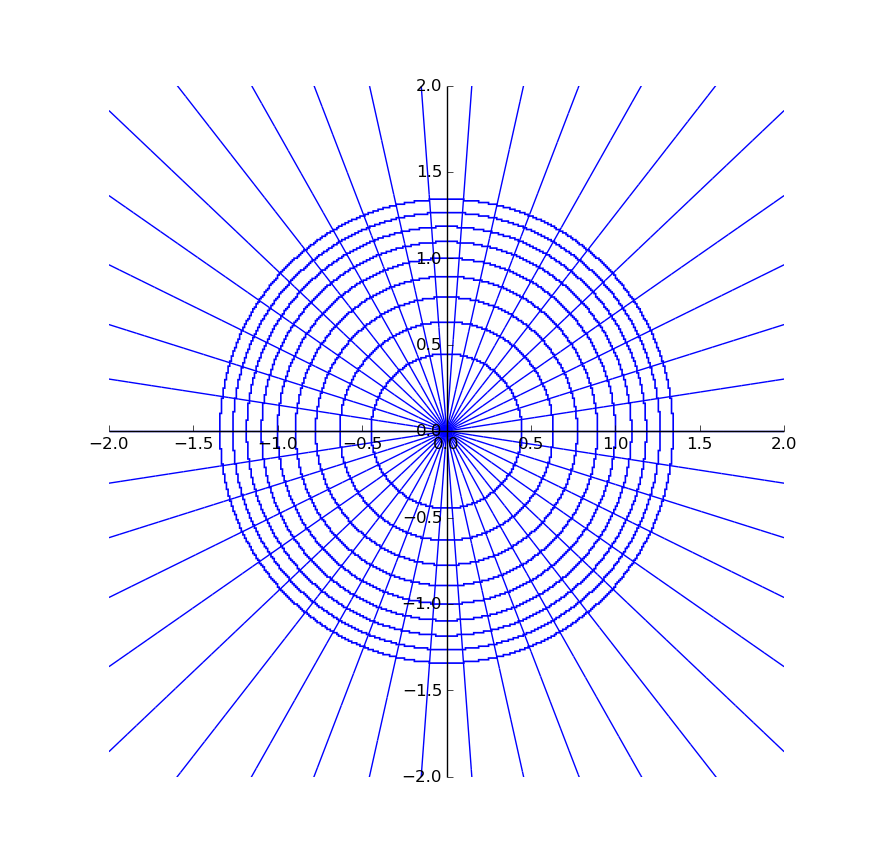
\includegraphics[scale=.2]{imagenes/flia_curvas_ortogonales.png}
\end{center}
\caption{Familia curvas ortogonales}\label{fig:ortogonales}
\end{figure}


\begin{problema}[Familias paramétricas de funciones en coordenadas polares]
En ocasiones la ecuación de la familia de curvas esta dada en otras coordenadas. Por ejemplo supongamos que tenemos la flia de curvas dadas por una EDO en coordenadas polares
\[\frac{dr}{d\theta}=f(r,\theta)\label{eq:flia_curvas_polar},\]
y queremos hallar su flia ortogonal.
\end{problema}

\noindent\textbf{Solución:} Calculemos $dy/dx$ para las curvas en la familia dada.
\[\frac{dy}{dx}=\frac{dy/d\theta}{dx/d\theta}=\frac{r_{\theta}\sen\theta+r\cos\theta}{r_{\theta}\cos\theta-r\sen\theta}=\frac{f\sen\theta+r\cos\theta}{f\cos\theta-r\sen\theta},\]

donde $r_{\theta}=dr/d\theta$. La flia ortogonal tiene que satisfacer

\[\frac{dy}{dx}=-\frac{f\cos\theta-r\sen\theta}{f\sen\theta+r\cos\theta}\]
Luego
\[\frac{r_{\theta}\sen\theta+r\cos\theta}{r_{\theta}\cos\theta-r\sen\theta}=-\frac{f\cos\theta-r\sen\theta}{f\sen\theta+r\cos\theta}.\]
Si despejamos $r_{\theta}$ llegamos a la ecuación de la flia de curvas ortogonales en coordenadas polares

\boxedeq{\frac{dr}{d\theta}=-\frac{r^2}{f}.}{eq_flia_ortogonal_polares}




\section{Separación de variables}

\begin{definicion}[Ecuaciones en variables separadas] Se dice que en una ecuación de primer orden
 \[y'=f(x,y)\]
 separan las variables, si es posible la factorización $f(x,y)=g(x)h(y)$.
\end{definicion}



Una ecuación  en la que se separan variables se puede resolver siguiendo los siguientes pasos. Como, asumiendo $h(y)\neq 0$,
\[\frac{y'}{h(y)}=g(x),\]
Si $H$ y $G$ son primitivas de $1/h$ y $g$ respectivamente por la regla de la cadena tenemos
\[\frac{d}{dx}H(y)=\frac{d}{dx}G(x)\]
Luego 
\[H(y)=G(x)+C,\quad C\in\rr.\]
Por último, si podemos encontrar la inversa de $H$
\boxedeq{y(x)=H^{-1}\left(G(x)+C\right).}{eq:var_sep}
será candidata a solución general. No podemos estar seguros de esta afrirmación, sobre todo porque la deducción de esta fórmula estuvo sujeta a suposiciones, como $h(y)\neq 0$.



\begin{ejemplo} Resolver
\[y'=\frac{y}{x}.\]
Es común emplear el método de la siguiente forma
\[\begin{split}
   \frac{dy}{dx}=\frac{y}{x} &\Longrightarrow \frac{dy}{y}=\frac{dx}{x} \Longrightarrow \int \frac{dy}{y}=\int \frac{dx}{x}\\
   &\Longrightarrow\ln|y|=\ln|x|+C \Longrightarrow |y|= k|x|, \hbox{ con }k>0\\
   &\Longrightarrow y= kx, \hbox{ con }k\in\rr
  \end{split}
\]
\end{ejemplo}




\begin{codigo}{\texttt{classify\_ode}: clasificación de ecuaciones}

\textbf{Sintaxis}\\
\texttt{classify\_ode(eq, f(x))}\\

\end{codigo}
\begin{ejemplo}

\end{ejemplo}

\begin{lstlisting}
x=symbols('x')
y=Function('y')(x)
MiEcua=Eq(y.diff(x),y/x)
tipo=classify_ode(MiEcua,y)
\end{lstlisting}
\textbf{Resultado:}\\
\begin{verbatim}
('separable', '1st_exact', '1st_linear', 
'almost_linear', 'lie_group',  etc)
\end{verbatim}




\section{Galeria de Ejemplos}

Vamos a describir algunos ejemplos. algunos de ellos llevan a problemas matemáticos muy simples. No obstante es oportuno discutirlos por dos motivos, habituarnos a la utilización de la matemática para resolver problemas de otras ciencias y sentar las bases para discutior problemas más relevantes desde una óptica matemática.

\subsection{Ley de reproducción normal}
  En muchos ejemplos de biología, química-física, etc, hay magnitudes que crecen(decrecen) siguiendo una ley que denominaremos
\href{http://es.wikipedia.org/wiki/Crecimiento_exponencial}{Ley de reproducción  normal}. Según esta ley la cantidad de individuos, sustancia, materia,
energía, etc, que se agrega o elimina de una población, cuerpo, etc por unidad de tiempo es proporcional a la cantidad de individuos, sustancia, etc que hay presente.   Una población de seres vivos puede reproducirse de esta manera bajo algunas circunstancias
especiales, por ejemplo si cuenta con fuente ilimitada de alimentos.

  Si $P(t)$ es la cantidad de individuos en el momento $t$, la ley de reproducción normal establece
en este caso la siguiente ecuación diferencial de primer orden
\[P'(t)=kP(t),\quad\text{ con } k>0.\]
La solución es hallada con suma facilidad, siendo ella 
\[\boxed{P(t)=Ce^{kt},\quad C\in\rr.}\]
La constante  $C$ se puede determinar si tenemos un problema a valores iniciales (pvi), por ejemplo $P(0)=P_0$, siendo $P_0\in\rr$ dado. En ese caso
$A=P_0$. 



  Otro ejemplo de comportamiento similar es la \href{http://es.wikipedia.org/wiki/Radiactividad}{desintegración radiactiva}. Algunos átomos de
ciertas sustancias, pueden ``desarmarse'' en átomos de otras sustancias. En el proceso suelen emitir radiaciones.  La velocidad de desintegración sigue una ley
de reproducción normal pero hay que tener en cuenta que la materia radiactiva, es decir la ``población''  en este caso, se pierde. Si $x(t)$ es la masa de materia radiactiva en el momento $t$, evolucionará
acorde a la ley
\[\boxed{x'(t)=-kx(t),\quad\text{con } k>0.}\]



\subsection{Soluciones}

\begin{problema}
\begin{tabular}{m{5cm} m{4.5cm}}
 Un tanque contiene inicialmente $N$ $\hbox{m}^3$ de $H_2O$ entre los cuales hay disueltos $C$ kg de sal común
 $NaCl$. A través de una boca de entrada y una de salida empieza circular la solución, entrando y saliendo al mismo caudal $q\frac{\hbox{m}^3}{s}$. Se supone que 
 la solución entrante tiene una concentración conocida $r$. Encontrar la cantidad de sal en el momento $t$. &
  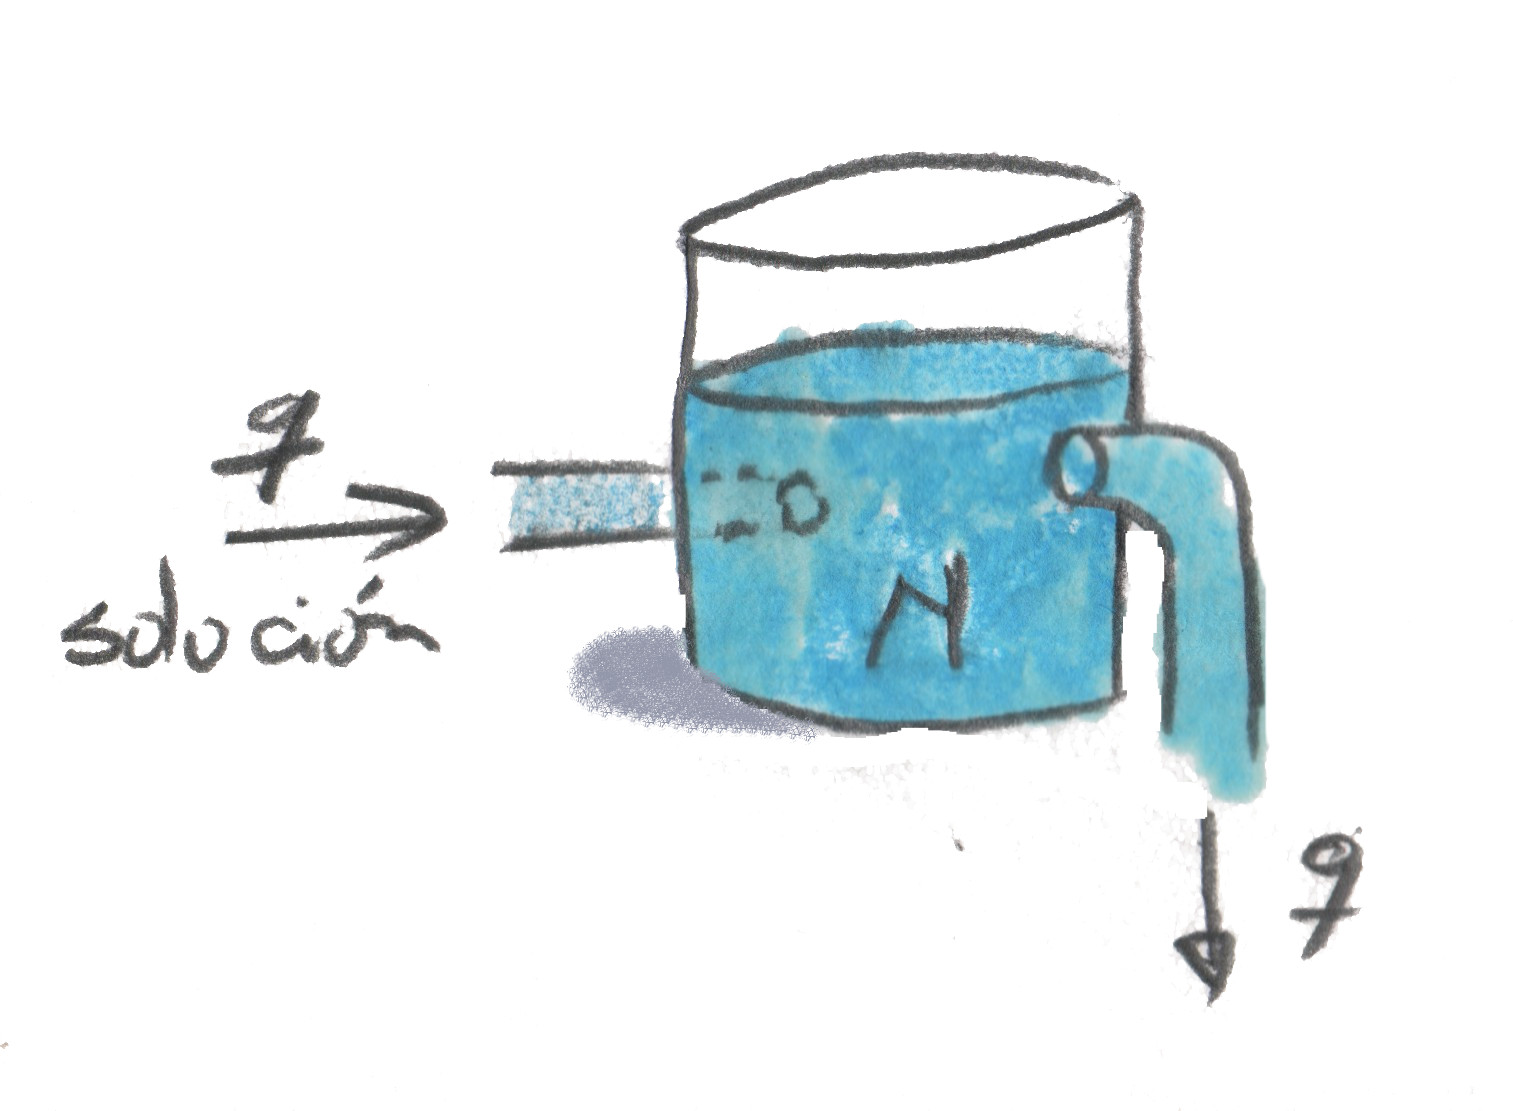
\includegraphics[scale=.1]{imagenes/tanque.jpg} \\
\end{tabular}
\end{problema}


 Sea $x(t)$ la cantidad de $NaCl$ en el tanque en el momento $t$. entonces

\[\begin{split}
   x'(t)&=\text{cantidad que entra }-\text{cantidad que sale }\\
          &=qr-q\frac{x(t)}{N}
  \end{split}
\]




\subsection{Dinámica del punto}

\subsubsection{Discusión Teórica}
Vamos a recordar algunas temas de la asignatura física. En particular  el movimiento de un cuerpo de masa $m$ al que podemos suponer puntual. Lo llamaremos punto masa. Denotamos por $x(t)$ su posición, digamos en $\rr^3$. Suponemos
que sobre él actúa una fuerza $f$. Recordemos que $x'(t)$ es la velocidad $v(t)$ y que $x''(t)$ es la aceleración $a(t)$.  
\href{http://es.wikipedia.org/wiki/Leyes_de_Newton\#Segunda_ley_de_Newton_o_ley_de_fuerza}{La segunda ley de Newton} implica que 
\begin{equation}\label{2leyR}\boxed{mx''(t)=f}\end{equation}


Supongamos que el movimiento del punto masa se realiza entre los momentos $t_0$ y $t_1$. Como has visto en Cálculo III la lóngitud de la curva recorrida 
$s(t)$ se puede calcular por
\begin{equation}\label{2ley}s=\int_{t_0}^{t_1}|x'(t)|dt=\int_{t_0}^{t_1}|v(t)|dt.\end{equation}
A $s$ se lo suele denominar \href{http://es.wikipedia.org/wiki/Longitud_de_arco}{elemento de arco}. Es comun querer utilizar a $s$ como variable independiente en 
lugar de $t$, puesto que algunas fórmulas se simplifican de esta forma. Por ejemplo

\begin{equation}\label{pre_trab} f\cdot v(t)dt=f\cdot\frac{v(t)}{|v(t)|}|v(t)|dt=f_tds,\end{equation}
donde $f_t$ denota la proyección de la fuerza $f$ sobre la dirección tangente a la trayectoria.





Si integramos \eqref{pre_trab} entre $t_0$ y $t_1$ y usamos \eqref{2leyR} obtenemos
\[\begin{split} W:=\int_{s_0}^{s_1}f_t(x(s))ds&=\int_{t_0}^{t_1} f(x(t))\cdot v(t)dt\\
   & =m \int_{t_0}^{t_1} v'(t)\cdot v(t)dt\\
   &=\frac{m}{2} \int_{t_0}^{t_1} \frac{d|v|^2}{dt}dt\\
   &=\frac{m}{2}|v(t_1)|^2-\frac{m}{2}|v(t_0)|^2.  \end{split}\]


  A la cantidad $\frac{m}{2}|v|^2$ se la denomina \emph{energía cinética} $E_c$ y a $W$ se lo denomina \emph{trabajo}.
Las relaciones obtenidas dicen que la variación de la energía cinética es igual al trabajo realizado $W=\Delta E_c$ por la fuerza $f$.
El trabajo realizado depende de la proyección tangencial de la fuerza $f_t$.  Llamaremos a esta relación
\href{https://es.wikipedia.org/wiki/Conservaci%C3%B3n_de_la_energ%C3%ADa}{Principio de Conservación de la Energía Mecánica.}

  Vamos a referirnos por \emph{rapidez} al módulo de la velocidad.
Si uno quiere incrementar o reducir la rapidez final $|v(t_1)|$ entonces deberá tener fuerzas con una componente tangencial no nula. 
Dicho de otra forma, si la fuerza es perpendicilar al movimiento, no hay cambio de rapidéz. 

  Hay fuerzas que siempre actuan en la dirección del movimiento. El ejemplo más conocido son las fuerzas de fricción, resistencia del aire,
resistencia a la rodadura, etc. Estás fuerzas, actúan sólo en la dirección del movimiento y se oponen a él.


 

  Por el contrario hay otras que actúan perpendiculares al movimiento $f_t=0$. Ejemplo de ello son las fuerzas que mantienen a un cuerpo moviéndosé a lo largo
de una guía. Por ejemplo un niño cayendo por un tobogan. Que el niño no se despegue de la guía (tobogán) se explica por la aparición de una fuerza que se denomina
reacción de vínculo que actúa en la dirección perpendicular al movimiento esto es decir a la guía. Está fuerza debe compensar a toda otra fuerza que trata de apartar
al cuerpo de la guía.  En el caso del tobogán la gravedad trata de apartar al niño de aquel.





\subsubsection{Cuerpos cayendo por guías}
Analicemos más en detalle el movimiento de un cuerpo cayendo a lo largo de una guía estando además influído  por la acción de la gravedad. Supondremos el movimiento en las proximidades de la superficie de la Tierra y por ello, supondremos que la fuerza de la gravedad es la constante $mg$. 

\begin{tabular}{m{5cm} m{4.5cm}}
 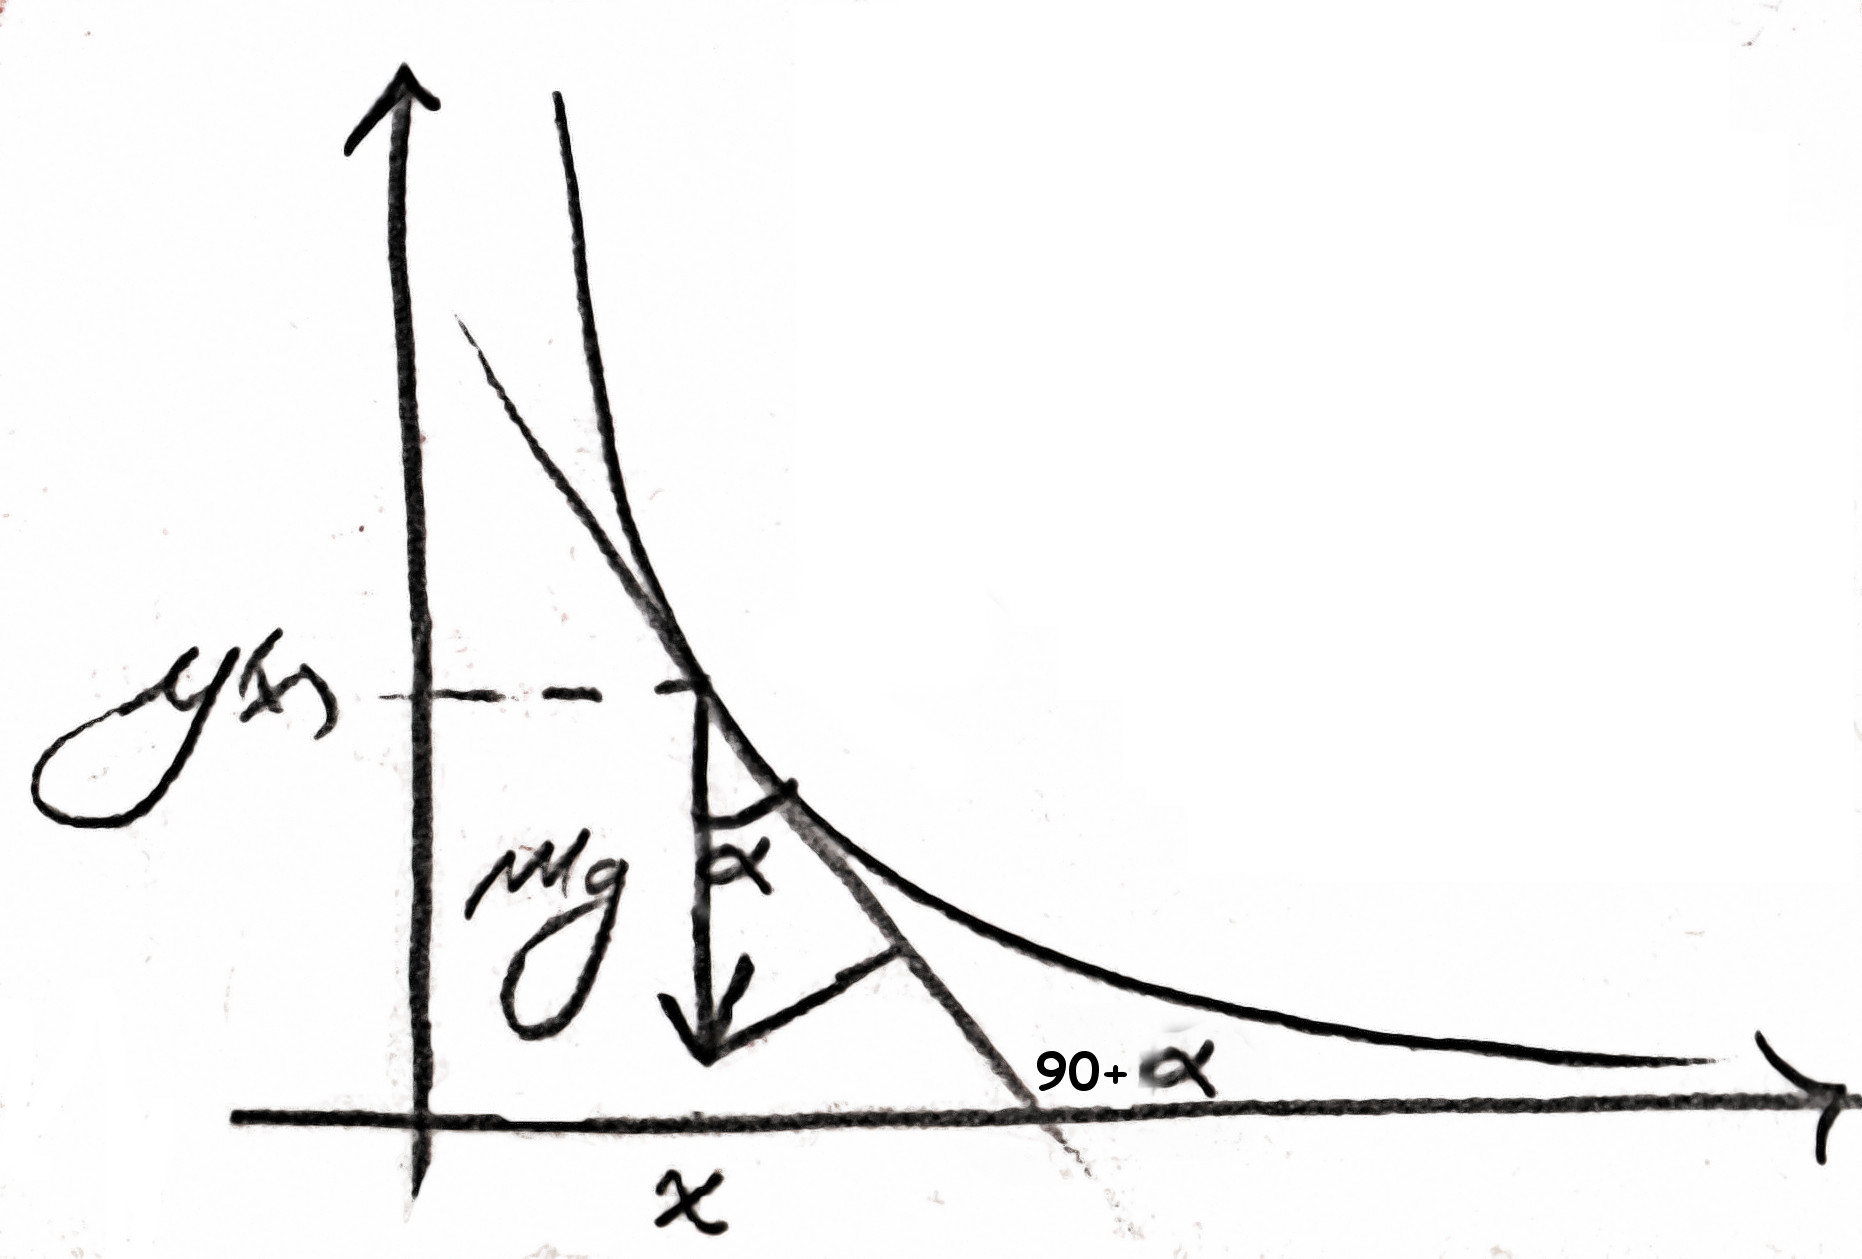
\includegraphics[scale=.07]{imagenes/caida_guia.jpg} & Supongamos que la guía esta
confinada a un plano. Introducimos un sistema de coordenadas ortogonales en dicho plano, con el suelo paralelo al eje $x$
\end{tabular}

El elemento longitud de arco $s$ de una curva que es el gráfico de una función $y(x)$ para $x$ en $[x_0,x_1]$ viene dado por 
\[s=\int_{x_0}^{x_1}\sqrt{1+y'(x)^2}dx\]
La fuerza de vínculo de la guía tiene componente tangencial nula,  la gravedad tiene una componente tangencial no nula. 
Su magnitud es $mg\cos\alpha$ (ver dibujo). Vamos a tratar de expresar $\cos\alpha$  en términos de   $y'(x)$. Vamos a suponer $\cos\alpha>0$ e $y'(x)<0$. 
Los demás casos quedan como \textbf{ejercicio}.
\[ \tan^2\alpha=\frac{\sen^2\alpha}{\cos^2\alpha}=\frac{1-\cos^2\alpha}{\cos^2\alpha}=\frac{1}{\cos^2\alpha}-1\]
y
\[y'(x)=\tan \left(\frac{\pi}{2}+\alpha\right)=-\frac{1}{\tan\alpha}\]
Podemos usar las relaciones anteriores para escribir $\cos\alpha$ en función de $y'(x)$
\begin{equation}\label{cos_alpha}\cos\alpha=-\frac{y'(x)}{\sqrt{1+y'(x)^2}}\end{equation}
Entonces
\begin{equation}\label{cons_ener}
 \begin{split} \frac{m}{2}|v(t_1)|^2-\frac{m}{2}|v(t_0)|^2&=\int_{s_0}^{s_1}f_tds =\int_{x_0}^{x_1}f_t\frac{ds}{dx}dx\\
&= -mg\int_{x_0}^{x_1}\frac{y'(x)}{\sqrt{1+y'(x)^2}}\sqrt{1+y'(x)^2}dx\\
&=-mg\left(y_1-y_0\right)
    \end{split}\end{equation}
Esto nos permite escribir la rapidez en función de la altura repecto al piso.




\begin{ejemplo}[Péndulo]
\end{ejemplo}

\noindent\begin{tabular}{m{6cm} m{5.5cm}}
  Se trata de una masa puntual $m$ suspendida de un punto por medio de una barra de longitud $l$
 a la que suponemos sin masa. Equivale al movimiento sobre una guía circular.  Usaremos el ángulo $\alpha$ marcado en la figura, como variable dependiente.
 & 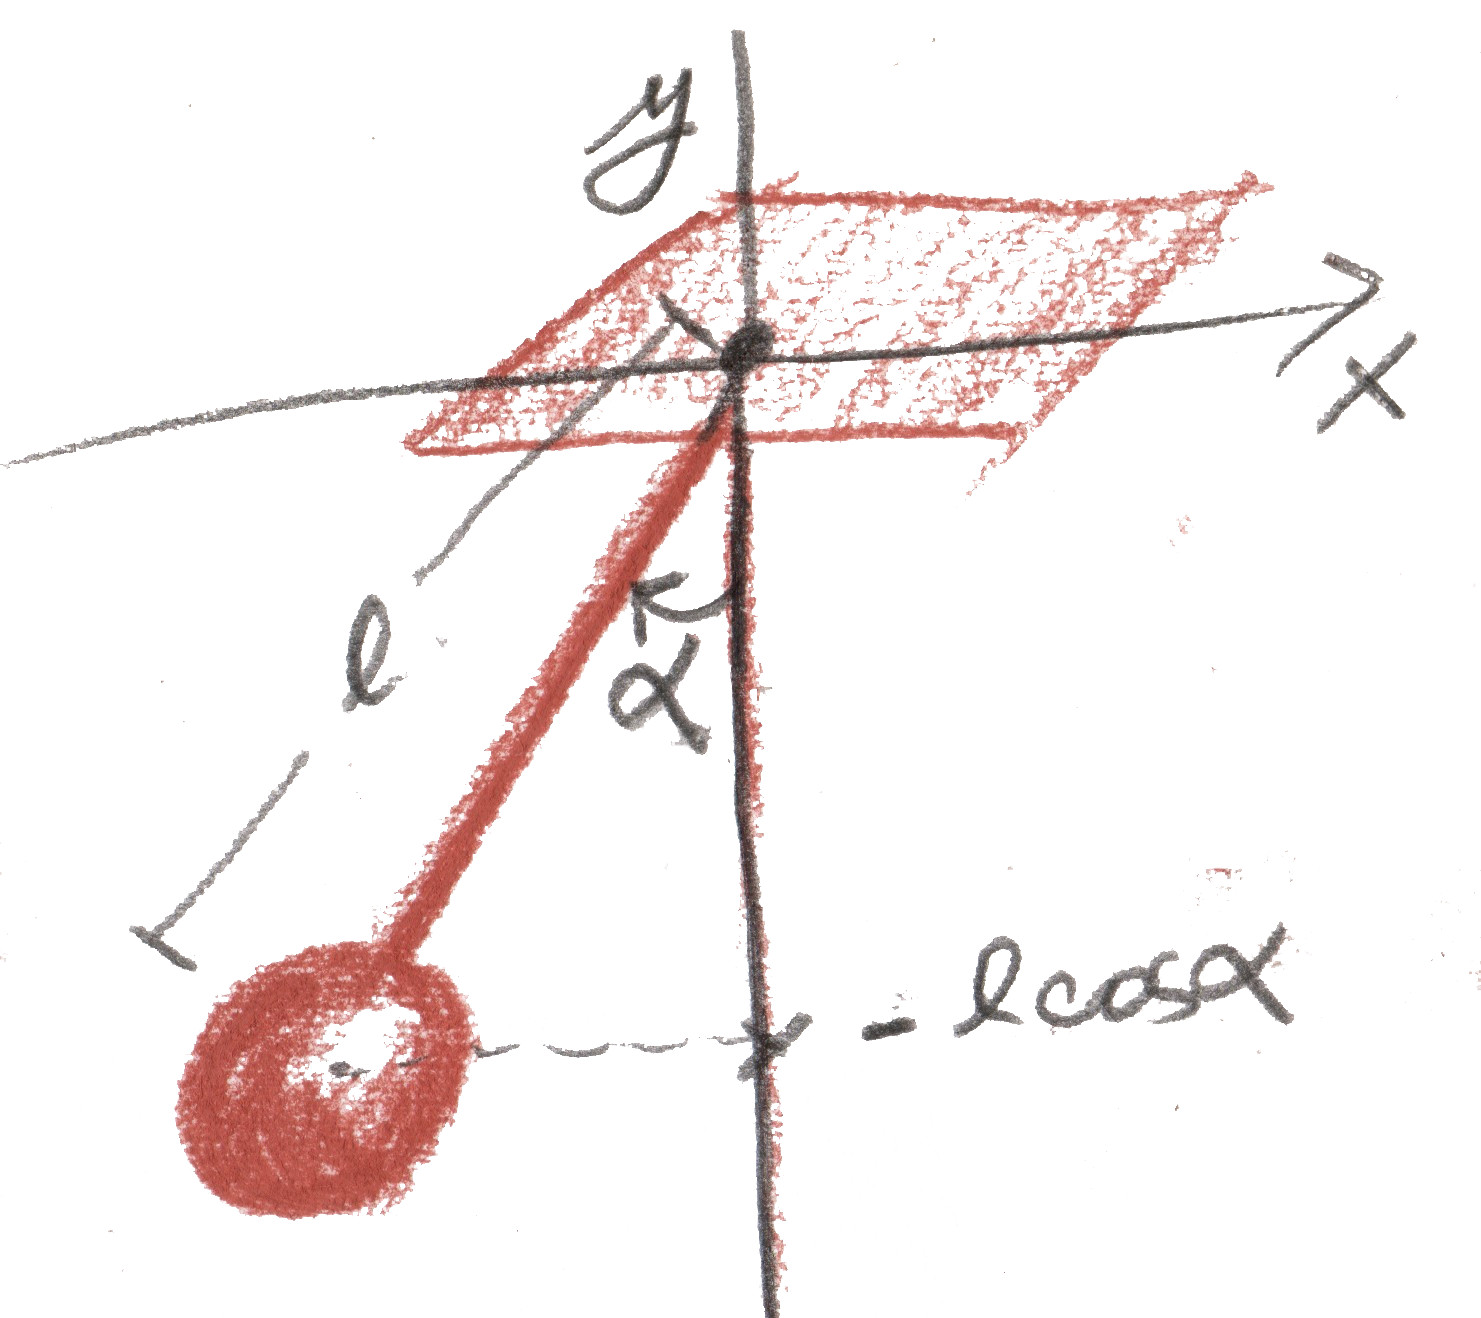
\includegraphics[scale=.07]{imagenes/pendulo.jpg} \\
\end{tabular}

Supondremos que el origen del sistema de de coordenadas está sobre el punto de amarre de la barra. Entonces de \eqref{cons_ener} con $t_1=t$ deducimos 
\[\begin{split}\frac{m|v(t)|^2}{2}-\frac{m|v(t_0)|^2}{2}&=-mg\left(y(t)-y(t_0)\right)\\
  &=mg\cos\alpha(t)-mg\cos\alpha(t_0).
   \end{split}
\]



Ahora la posición de la masa es $x(t)=l(\sen\alpha,-\cos\alpha)$ luego 
\[v(t)=l\alpha'(t)(\cos\alpha,\sen\alpha) \Longrightarrow |v(t)|^2=l^2\alpha'(t)^2.\]
Entonces
\[\frac{ml^2\alpha'(t)^2}{2}= mgl\cos\alpha(t)-mgl\cos\alpha(t_0) +\frac{mv(t_0)^2}{2}.\]
Derivando esta relación
\[ml^2\alpha'(t)\alpha''(t)=-mgl\alpha'(t)\sen\alpha(t).\]
De esto deducimos la ecuación del \href{http://es.wikipedia.org/wiki/Péndulo}{péndulo}
\[\boxed{\alpha''(t)=-\frac{g}{l}\sen\alpha(t)}.\]


\begin{ejemplo}[La braquistócrona]

\end{ejemplo}


\begin{problema} Dados dos puntos $A$ y $B$ en las proximidades de la superficie terrestre, uno mas abajo respecto al suelo que el otro,
queremos diseñar el tobogán óptimo entre los dos,
esto es el tobogán que nos lleve de $A$ hasta $B$ en el menor tiempo. La curva solución a este problema se llama curva 
\href{http://es.wikipedia.org/wiki/Curva_braquistócrona}{braquistócrona} (braquistos - el más corto, cronos - tiempo). 
\end{problema} \marginpar{\vspace{-30mm}
 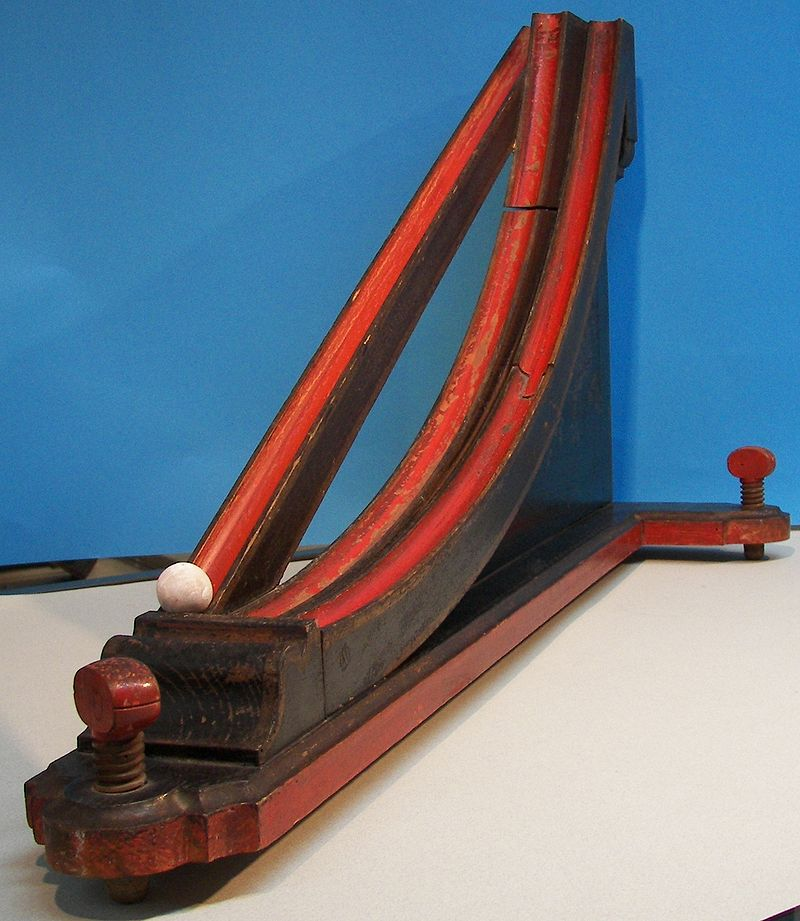
\includegraphics[scale=.07]{imagenes/braquis.jpg}
}
% \begin{center}


 Este problema fue resuelto por primera vez por Johann Bernoulli y es unos de los problemas precursores de la rama de las matemáticas que se denomina
\href{http://es.wikipedia.org/wiki/Cálculo_variacional}{cálculo de 
variaciones}. Vamos a dar la solución de Bernoulli que es muy elegante y está basada en un resultado de óptica llamado 
 el \href{http://es.wikipedia.org/wiki/Principio_de_Fermat}{Principio de Mínimo Tiempo} de \href{http://es.wikipedia.org/wiki/Fermat}{Fermat}.

\begin{boite}[boxcolor=orange, background=blue!5, titlebackground=blue!20,
titleboxcolor = black]{\href{http://es.wikipedia.org/wiki/Principio_de_Fermat}{\textbf {Principio de Mínimo Tiempo}} \textbf{de} \href{http://es.wikipedia.org/wiki/Fermat}{\textbf{Fermat}}}
 La luz sigue para ir de un punto a otro el recorrido que minimiza el tiempo.
\end{boite}



 La primera impresión   es que ese reccorrido debería ser la línea recta. Si embargo esto no es así debido a que la velocidad de la luz cambia
de acuerdo al \href{http://es.wikipedia.org/wiki/Velocidad_de_la_luz_en_un_medio_material}{medio que atraviesa}. 
La velocidad de la luz en el vacío es 299.792,458km/h y en el diamante 124.034,943 km/h. La velocidad de la luz cambia no sólo con la sustancia sino con sus cualidades, 
como la densidad. 

 Si la luz se mueve dentro de un medio homogéneo, el camino que sigue es la línea recta. Esto ya no es más así cuando la luz cambia de medio de propagación. Por ejemplo
cuando pasa del aire al vidrio. 


\begin{tabular}{m{4cm} m{7.5cm}}
 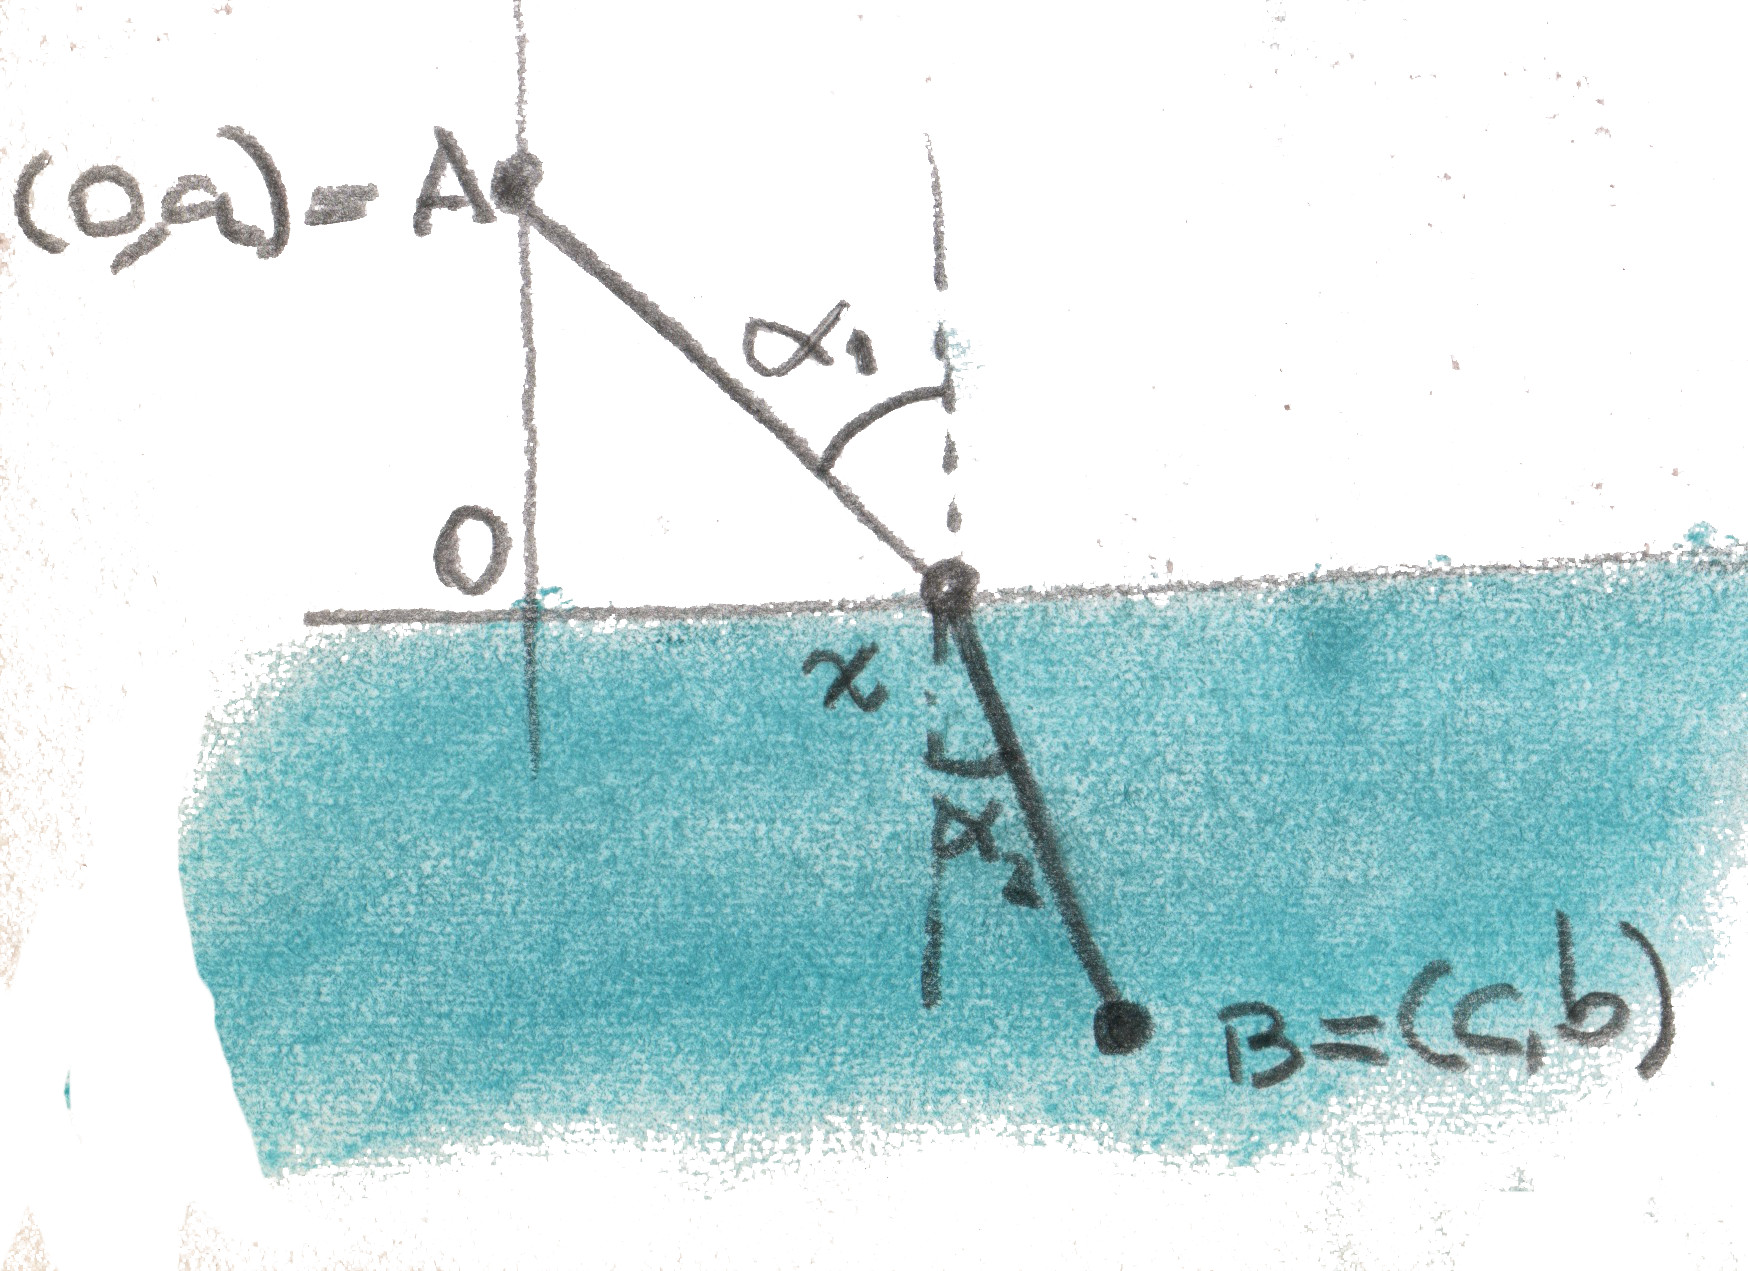
\includegraphics[scale=.07]{imagenes/refraccion.jpg} & Supongamos que la luz une los puntos $A$ y $B$ del plano y en el camino atravieza de un medio a otro, siendo la velocidad
 de la luz en cada uno de ellos $v_1$ y $v_2$.  Supongamos que $A=(a,0)$ y $B=(c,b)$ y el eje $x$ es la frontera entre los medios.
 \end{tabular}
Como sabemos que mientras se mueva en un medio homogéneo la luz sigue en línea recta,
el tiempo que emplea la luz para ir $A$ a $B$ es
 \[t=\frac{\sqrt{a^{2} + x^{2}}}{v_{1}} + \frac{\sqrt{{\left(c - x\right)}^{2} + b^{2}}}{v_{2}}\]
Para determinar la trayectoria es suficiente encontrar $x$, el punto donde la luz choca con la interfaz entre los medios. 
El principio de Fermat afirma que el tiempo es mínimo de modo que hallaremos un punto crítico de $t$ respecto a $x$. 
\[ \frac{dt}{dx}=-\frac{c - x}{\sqrt{{\left(c - x\right)}^{2} + b^{2}} v_{2}} +
\frac{x}{\sqrt{a^{2} + x^{2}} v_{1}}=\frac{\sen\alpha_1}{v_1}-\frac{\sen\alpha_2}{v_2} \]
Deducimos que en un punto crítico 
\boxedeq{\frac{\sen\alpha_1}{v_1}=\frac{\sen\alpha_2}{v_2} }{eq:ley_snell1}
que se denomina \href{http://es.wikipedia.org/wiki/Ley_de_Snell}{Ley de Snell}. El punto crítico es mínimo pues $\left.\frac{dt}{dx}\right|_{x=0}=-\tfrac{c}{bv_2}<0$ y
$\left.\frac{dt}{dx}\right|_{x=c}=\tfrac{c}{\sqrt{c^2+a^2}v_1}>0$.

 A la razón entre la velocidad de la luz dentro de un determinado medio y la velocidad de la luz en el vacio se lo denomina
\href{http://es.wikipedia.org/wiki/Índice_de_refracción}{índice de refracción} y se lo denota con la letra $n$. La Ley de Snell se la suele escribir
\[\boxed{n_1\sen\alpha_1=n_2\sen\alpha_2 }.\]
Que pasa si la luz atraviesa un medio que va cambiando de manera continua de índice de refracción. Por ejemplo, el índice de refracción en la atmósfera
va cambiando de manera continua con la altitud respecto a la superficie terrestre, ya que la densidad del aire va cambiando con la altitud. La Ley de
Snell en este caso es
\[\boxed{\frac{\sen\alpha}{v}=\text{cte}}\]
Aquí el ángulo $\alpha$ y la velocidad $v$ cambian respecto a alguna variable/s real/es, por ejemplo la altitud.


¿Que tienen en común el recorrido de la luz y la braquistócrona? Bernoulli se dió cuenta que la situación en los dos casos es la misma, ya que en los dos casos
se trata de minimizar el tiempo del recorrido. De modo que la braquistócrona también tiene que satisfacer la Ley de Snell.
 Ahora supongamos un sistema de coordenadas con origen en el punto $A$, inicial del recorrido.  Además supongamos que el movil  parte
del reposo. Con estas suposiciones $x(t_0)=0$ y $v(t_0)=0$. Por la conservación de la energía 
\[\frac{m}{2}|v(t)|^2=-mgy(t)=mg|y(t)|.\]
 Así por la ley de Snell
\[\frac{\sen\alpha}{|v(t)|}=\frac{\sen\alpha}{\sqrt{2g|y|}}=c=\text{ cte}.\]
En \eqref{cos_alpha} habíamos expresado el $\cos\alpha$ (en realidad del ángulo opuesto por el vértice, pero es igual) mediante la derivada. Luego
\[\sen\alpha=\sqrt{1-\cos^2\alpha}=\frac{1}{\sqrt{1+y'(x)^2}}.\]
Entonces tenemos
\[\sqrt{2g|y|}\sqrt{1+y'(x)^2}=c=\hbox{ cte}\]
Despejando llegamos a la ecuación diferencial
\[\boxed{\sqrt{\frac{y}{c-y}}y'=1}.\]
Es una ecuación con variables separables. La constante $c$ no tiene el mismo valor que en la ecuación anterior.  

La solución se obtiene resolviendo la integral
\[x=\int dx=\int \sqrt{\frac{y}{c-y}}dy.\]
lo que no es tan sencillo. Hacemos el cambio de variables
\[\sqrt{\frac{y}{c-y}}=\tan\phi\Longrightarrow y=c\sen^2\phi\Longrightarrow dy=2c\sen\phi\cos\phi d\phi.\]
Luego
\[x=2c\int\sen^2\phi d\phi=\frac{c}{2}\left(2\phi-\sen 2\phi\right)+C_1.\]
Como tiene que pasar por $x=0$ e $y=0$ debe ser $C_1=0$.  Tenemos que
 \[\left\{\begin{array}{l l l}
	      y&=c\sen^2 \phi&=\frac{c}{2}(1-\cos2\phi)\\
	      x&=\frac{c}{2}(2\phi-\sen2\phi)\ &\\
          \end{array}\right.
\]
Conviene llamar $2\phi=\theta$ y $a=c/2$
 \[\left\{\begin{array}{l l }
	      y&= a(1-\cos\theta)\\
	      x&=a(\theta-\sen\theta)\
          \end{array}\right.
\]
Que son la ecuaciones paramétricas de una curva conocida con el nombre de \href{http://es.wikipedia.org/wiki/Cicloide}{cicloide}. Podemos usar \texttt{SymPy} para graficar esta curva
\begin{lstlisting}
theta=symbols('theta')
from sympy.plotting import *
plot_parametric(theta-sin(theta),1-cos(theta),(theta,0,10*pi))
\end{lstlisting}

\begin{figure}[h]
\begin{center}
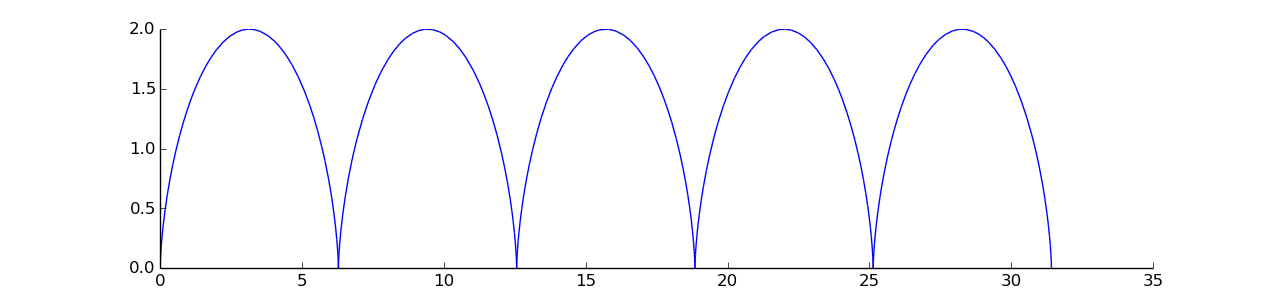
\includegraphics[scale=.3]{imagenes/cicloide.png}
\end{center}\caption{Cicloide}\label{fig:cicloide}
\end{figure}


Si in tentamos resolver las ecuaciones con \texttt{SymPy} el resultado no es muy alentador.

\begin{lstlisting}
x,c=symbols('x,c')
y=Function('y')(x)
MiEcua=Eq(y.diff(x),sqrt((c-y)/y))
f=dsolve(MiEcua,y,hint='separable')
\end{lstlisting}
\textbf{Resultado:}
\[
 \begin{cases} - i \sqrt{c} \sqrt{-1 + \frac{1}{c} y{\left (x \right )}} \sqrt{y{\left (x \right )}} - i c \operatorname{acosh}{\left (\frac{1}{\sqrt{c}} \sqrt{y{\left (x \right )}} \right )} & \text{for}\: \left\lvert{\frac{1}{c} y{\left (x \right )}}\right\rvert > 1 \\ \- \frac{\sqrt{c} \sqrt{y{\left (x \right )}}}{\sqrt{1 - \frac{1}{c} y{\left (x \right )}}} + c \operatorname{asin}{\left (\frac{1}{\sqrt{c}} \sqrt{y{\left (x \right )}} \right )} + \frac{y^{\frac{3}{2}}{\left (x \right )}}{\sqrt{c} \sqrt{1 - \frac{1}{c} y{\left (x \right )}}} & \text{otherwise} \end{cases} = C_{1} + x
\]




  \begin{ejemplo}[La tautócrona]


  \end{ejemplo}




  Vamos a ver otra propiedad notable de la ciclode. Supongamos que dejamos caer el cuerpo del reposo desde un punto intermedio, digamos en $(x_0,y_0)$. Sea  $\theta_0$
 el valor del paŕámetro $\theta$ correpondiente a este punto. ¿Cuánto tardara en llegar el cuerpo al punto mínimo de la curva que ocurre cuando $\theta=\pi$? 
% \begin{center}
% \animategraphics[controls,scale=.5]{15}{tautocrona/tauto-}{0}{79}
% \end{center}


  
  

 Tenemos
\[
 \left\{ \begin{array}{l l}
 \frac{dx}{d\theta}&=a(1-\cos\theta)\\
 \frac{dy}{d\theta}&=a\sen\theta 
 \end{array}\right.
\]
% 
Como el cuerpo ahora no parte de $(0,0)$ tendremos
\[|v|=\sqrt{2g(y_0-y)}.\]


  
  {La tautócrona}
Por \eqref{2ley} $ds/dt=|v|$. Si llamamos $T$ al tiempo que demanda en llegar a $\theta=\pi$, y llamamos  $s_0$ y $s_1$ a los arcos correspondientes al punto inicial
y final.  Tenemos
 \[T=\int_0^Tdt=\int_{s_0}^{s_1}\frac{dt}{ds}ds=\int_{s_0}^{s_1}\frac{1}{\sqrt{2g(y_0-y)}}ds.\]
Cambiando la variable de integración a $\theta$. Como 
\[
 \frac{ds}{d\theta}=\sqrt{\left(\frac{dx}{d\theta}\right)^2+\left(\frac{dy}{d\theta}\right)^2}=\sqrt{2}a\sqrt{1-cos\theta}.
\]
 Tenemos
\[T=\sqrt{\frac{a}{g}}\int_{\theta_0}^{\pi}\frac{\sqrt{1-\cos\theta}}{\cos\theta_0-\cos\theta}d\theta=
\sqrt{\frac{a}{g}}\int_{\theta_0}^{\pi}\frac{\sen\frac{\theta}{2}}{\cos^2\frac{\theta_0}{2}-\cos^2\frac{\theta}{2}}d\theta.
\]
Ahora hacemos la sustitución
\[u=\frac{\cos\frac{\theta}{2}}{\cos\frac{\theta_0}{2}}\Longrightarrow du=-\frac{\sen\frac{\theta}{2}}{2\cos\frac{\theta_0}{2}}d\theta.\]
Vemos que
\[
 T=2\sqrt{\frac{a}{g}}\int_0^1\frac{1}{\sqrt{1-u^2}}du.
\]
Que es una expresión independiente de $\theta_0$. En consecuencia el tiempo $T$ que demanda  el cuerpo para llegar $\theta=\pi$ es siempre el mismo no importa
desde donde se deje caer.



\end{document}